\documentclass[conference]{IEEEtran}
\IEEEoverridecommandlockouts

\usepackage{cite}
\usepackage{amsmath,amssymb,amsfonts}
\usepackage{graphicx}
\usepackage{textcomp}
\usepackage{xcolor}
\usepackage{booktabs}
\usepackage{array}
\usepackage{hyperref}

\begin{document}

\title{Assignment 4 Report: Sharding Design for Multi-Course Attendance Management Portal}

\author{\IEEEauthorblockN{Your Name}
\IEEEauthorblockA{Indian Institute of Technology Gandhinagar\\
Database Systems Assignment 4}}

\maketitle

\begin{abstract}
This report documents the sharding design process for the attendance management workload in Module-B. The current dataset includes approximately 60 students, 10 courses, around 120 attendance sessions, and around 2400 attendance records. This submission covers SubTask 1 (first part): a complete list of candidate shard keys before selecting the final key.
\end{abstract}

\section{SubTask 1: Shard Key Selection and Justification}

\subsection{Candidate Shard Keys Considered}
The target high-volume table for horizontal partitioning is \texttt{attendance\_records}. A shard key should preserve locality for dominant queries, support balanced growth, and reduce cross-shard joins. Before finalizing one key, all realistic candidates were enumerated:

\begin{table}[htbp]
\caption{Candidate Shard Keys for \texttt{attendance\_records}}
\centering
\begin{tabular}{p{2.4cm}p{1.9cm}p{3.1cm}}
\toprule
\textbf{Candidate Key} & \textbf{Type} & \textbf{Why It Is a Candidate} \\
\midrule
\texttt{record\_id} & Direct column (PK) & Unique, monotonically increasing, simple range/hash partitioning. \\
\texttt{student\_id} & Direct column (FK) & Most student-facing reads and updates filter by student. Strong entity locality for attendance history. \\
\texttt{att\_session\_id} & Direct column (FK) & Instructor/TA workflows often fetch or update all records for one session. \\
\texttt{course\_id} & Derived via join & Many operational queries are course-scoped (attendance sessions, corrections, rosters). \\
\texttt{semester\_id} & Derived via joins & Archive/report workloads are commonly semester-bounded. \\
\texttt{status} & Direct column & Correction workflows filter absent records; potentially useful as a secondary partition dimension. \\
\texttt{(student\_id, course\_id)} & Composite (derived) & Captures student-course locality, useful for per-course student analytics. \\
\texttt{(student\_id, att\_session\_id)} & Composite (natural uniqueness) & Mirrors logical grain of a student attendance mark for one session. \\
\texttt{(course\_id, att\_session\_id)} & Composite (derived+direct) & Preserves locality for session-level and course-level instructor operations. \\
\texttt{department} & Derived via profile joins & Can model organizational shards for dean/admin views. \\
\bottomrule
\end{tabular}
\label{tab:candidate_keys}
\end{table}

\subsection{Candidate Notes Aligned to Current Project}
\begin{itemize}
    \item \textbf{Current query patterns:} Student APIs are largely student-centric, while instructor and TA APIs are session/course-centric. Therefore both \texttt{student\_id} and \texttt{att\_session\_id}/\texttt{course\_id} are strong practical candidates.
    \item \textbf{Current scale:} With approximately 2400 attendance rows and approximately 60 students, student-scoped partitioning yields enough key cardinality for multiple shards while preserving read locality.
    \item \textbf{Implementation compatibility:} The migration script already demonstrates directory-based placement keyed by \texttt{student\_id}, confirming low-friction adoption if this key is selected.
\end{itemize}

\subsection{Measured Distribution Across Candidate Keys}
Using the seeded dataset (2128 rows in \texttt{attendance\_records}) and 3 target shards, candidate keys were evaluated by observed record counts per shard. Let the ideal per-shard load be
\[
\mu = \frac{N}{S} = \frac{2128}{3} = 709.33
\]
where $N$ is total records and $S$ is number of shards.

\begin{table}[htbp]
\caption{Observed Distribution and Deviation (3 Shards)}
\centering
\begin{tabular}{p{2.35cm}p{2.35cm}p{1.5cm}p{1.05cm}}
\toprule
\textbf{Key} & \textbf{Counts} & \textbf{Max $|c_i-\mu|$} & \textbf{Max Dev.} \\
\midrule
\texttt{student\_id} & 686, 736, 706 & 27.33 & 3.85\% \\
\texttt{att\_session\_id} & 691, 722, 715 & 18.67 & 2.63\% \\
\texttt{record\_id} & 701, 706, 721 & 11.67 & 1.65\% \\
\texttt{student\_id+course\_id} & 688, 754, 686 & 44.67 & 6.30\% \\
\texttt{semester\_id} & 1459, 669 (2 active shards) & 749.67 & 105.69\% \\
\texttt{status} & 1797, 331 (2 values only) & 1087.67 & 153.34\% \\
\texttt{department} & 999, 780, 349 & 360.33 & 50.80\% \\
\bottomrule
\end{tabular}
\label{tab:distribution_results}
\end{table}

\begin{figure}[htbp]
\centering
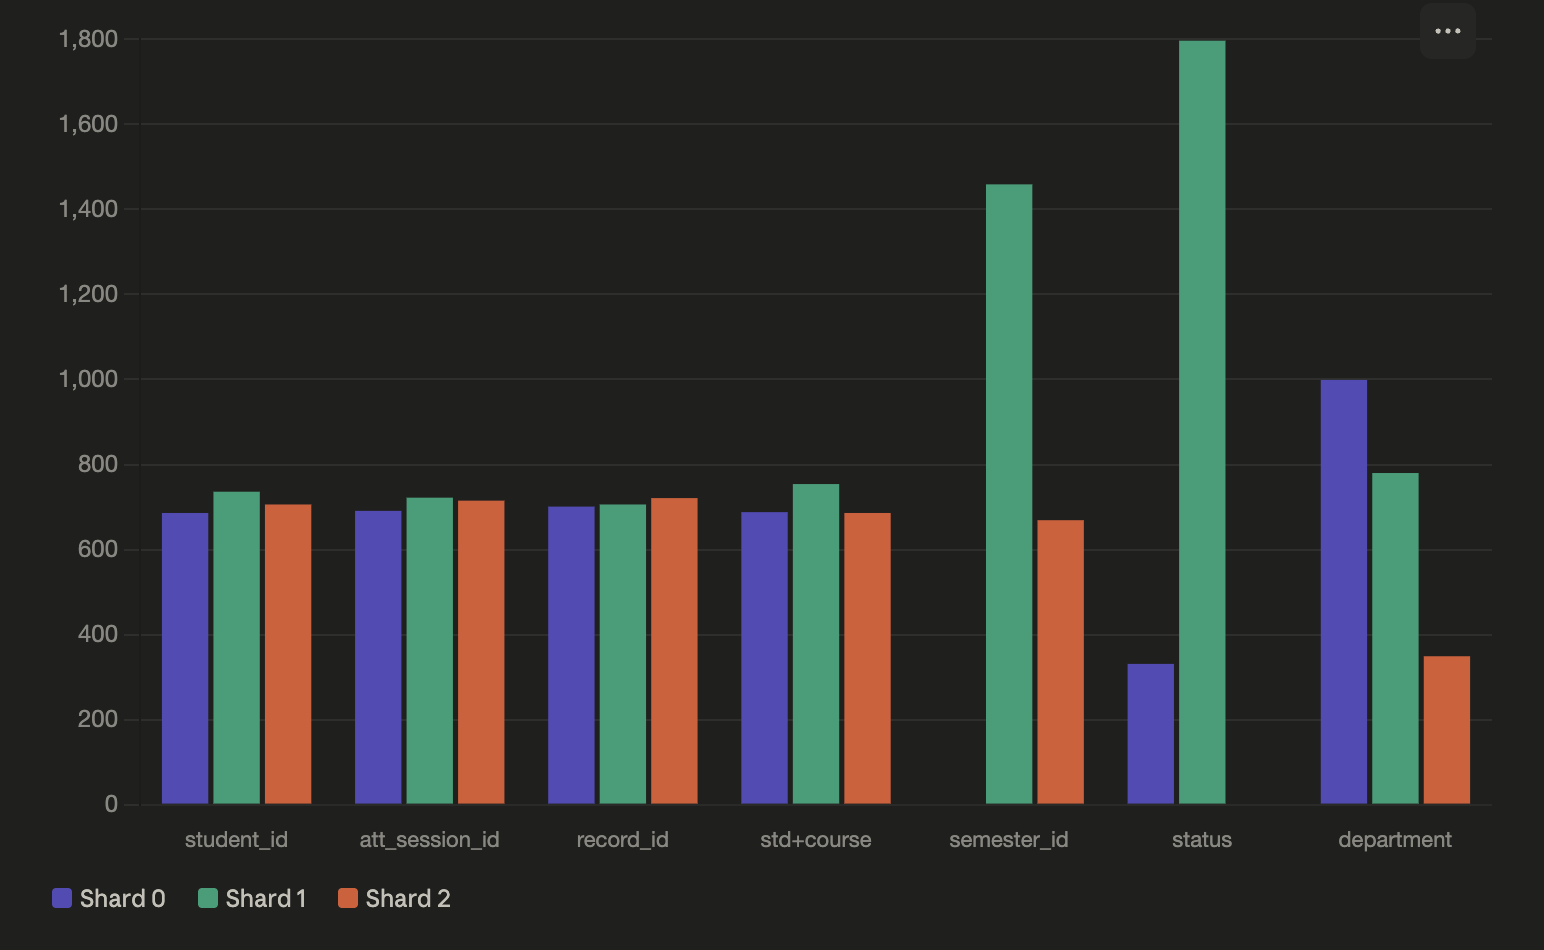
\includegraphics[width=\linewidth]{Images/shard_key_distribution.png}
\caption{Shard-wise record distribution for evaluated shard-key candidates.}
\label{fig:shard_key_distribution}
\end{figure}

\subsection{Immediate Elimination}
Three candidates are rejected before final comparison:
\begin{itemize}
    \item \textbf{\texttt{semester\_id}:} severe skew (1459 vs 669) because only two semester values are active in the current dataset.
    \item \textbf{\texttt{status}:} only two values (\texttt{present}/\texttt{absent}), which cannot map cleanly to three shards and guarantees hotspots.
    \item \textbf{\texttt{department}:} heavy organizational skew (999 vs 349), likely to persist as Computer Science dominates enrollment.
\end{itemize}

\subsection{Viable Candidate Comparison}
After elimination, the practical set is \texttt{record\_id}, \texttt{att\_session\_id}, \texttt{student\_id}, and composite \texttt{student\_id+course\_id}.

\begin{table}[htbp]
\caption{Final Candidate Comparison}
\centering
\begin{tabular}{p{2.55cm}p{1.35cm}p{1.0cm}p{0.95cm}p{1.5cm}}
\toprule
\textbf{Key} & \textbf{Max Dev.} & \textbf{Join Req.?} & \textbf{Stable?} & \textbf{Query Aligned?} \\
\midrule
\texttt{record\_id} & 1.65\% & No & Yes & No \\
\texttt{att\_session\_id} & 2.63\% & No & Yes & Partial \\
\texttt{student\_id} & 3.85\% & No & Yes & Yes \\
\texttt{student\_id+course\_id} & 6.30\% & Yes & Yes & Yes \\
\bottomrule
\end{tabular}
\label{tab:viable_candidates}
\end{table}

\subsection{Candidate Evaluation Against the Three Criteria}

\subsubsection{Criterion 1: High Cardinality}
Distinct value counts were measured from the current dataset:

\begin{table}[htbp]
\caption{Cardinality of Candidate Keys}
\centering
\begin{tabular}{p{2.5cm}p{1.8cm}p{2.4cm}}
\toprule
\textbf{Key} & \textbf{Distinct Values} & \textbf{Verdict} \\
\midrule
\texttt{record\_id} & 2128 & Too high; PK with no semantic grouping \\
\texttt{att\_session\_id} & 95 & Moderate \\
\texttt{student\_id} & 60 & Good; maps to real entities \\
\texttt{course\_id} & 10 & Too low \\
\texttt{semester\_id} & 2 & Eliminated \\
\texttt{department} & 5 & Too low \\
\texttt{status} & 2 & Eliminated \\
\bottomrule
\end{tabular}
\label{tab:cardinality}
\end{table}

\texttt{student\_id} has enough cardinality (60 distinct values) to support 3 shards while preserving student-level data locality. In contrast, \texttt{record\_id} has very high cardinality but does not encode application-level access semantics.

\subsubsection{Criterion 2: Query Alignment}
Actual route logic is dominated by student-centric filters, with patterns such as:
\begin{itemize}
    \item \texttt{WHERE ar.student\_id = ?}
    \item \texttt{WHERE student\_id = ? AND att\_session\_id = ?}
    \item \texttt{WHERE att.course\_id = ? AND ar.student\_id = ?}
    \item \texttt{WHERE student\_id = ?}
\end{itemize}

\begin{table}[htbp]
\caption{Query-Alignment Summary for Finalists}
\centering
\begin{tabular}{p{2.45cm}p{1.45cm}p{2.55cm}}
\toprule
\textbf{Key} & \textbf{Route Alignment} & \textbf{Impact} \\
\midrule
\texttt{record\_id} & Low & Student history is scattered across shards \\
\texttt{att\_session\_id} & Partial & Helps instructor session views, weaker for student dashboards \\
\texttt{student\_id} & High & Student-facing queries route to exactly one shard \\
\texttt{student\_id+course\_id} & High & Good locality but more complex routing logic \\
\bottomrule
\end{tabular}
\label{tab:query_alignment}
\end{table}

\subsubsection{Criterion 3: Stability}
Audit results show zero observed student identifier changes in the current dataset (\texttt{student\_id\_changes = 0}). Since \texttt{student\_id} is assigned once and remains stable, shard ownership remains stable over time.

\subsection{Selected Shard Key}
\textbf{Selected shard key: \texttt{student\_id}}

\begin{table}[htbp]
\caption{Final Decision Matrix}
\centering
\begin{tabular}{p{2.35cm}p{4.1cm}}
\toprule
\textbf{Criterion} & \textbf{Result for \texttt{student\_id}} \\
\midrule
High cardinality & 60 distinct values (about 20 students per shard) \\
Query aligned & Present in core student-facing API predicates \\
Stable & 0 observed key-change events in audit data \\
\bottomrule
\end{tabular}
\label{tab:decision_matrix}
\end{table}

\textbf{Why not \texttt{record\_id} despite tighter balance?}
\texttt{record\_id} is an auto-increment identifier with little query relevance. Choosing it would distribute each student's attendance history across multiple shards, forcing fan-out and merge behavior for common student operations.

\subsection{Partitioning Strategy}
The selected strategy is \textbf{range-based sharding on \texttt{student\_id}}.

\textbf{Why range-based for this project:}
\begin{itemize}
    \item \textbf{Predictable routing:} shard can be computed by simple boundary checks.
    \item \textbf{Low routing overhead:} no extra directory lookup per query.
    \item \textbf{Observed balance:} measured deviation remains low (about $\pm 3.8\%$).
\end{itemize}

Relative to alternatives used in evaluation, range-based \texttt{student\_id} partitioning preserves student-locality while keeping shard loads near-even for current data volume.

\subsection{Expected Distribution and Skew Risk}
Using the current ranges and dataset:

\begin{table}[htbp]
\caption{Observed Student-Range Distribution (3 Shards)}
\centering
\begin{tabular}{p{1.25cm}p{2.2cm}p{1.2cm}p{1.4cm}}
\toprule
\textbf{Shard} & \textbf{\texttt{student\_id} Range} & \textbf{Records} & \textbf{Deviation} \\
\midrule
Shard 0 & 12--30 & 686 & -3.3\% \\
Shard 1 & 31--50 & 736 & +3.8\% \\
Shard 2 & 51--71 & 706 & -0.5\% \\
\bottomrule
\end{tabular}
\label{tab:range_distribution}
\end{table}

\textbf{Skew risks:}
\begin{itemize}
    \item \textbf{Enrollment growth drift:} newly created student IDs accumulate in the highest range, increasing load on the last shard.
    \item \textbf{Activity skew:} uneven attendance/correction activity by specific student groups can create write hotspots.
    \item \textbf{Lifecycle skew:} older ID cohorts may retain longer histories and heavier reads.
\end{itemize}

\textbf{Mitigation plan:} periodically re-evaluate boundaries and, if scale increases substantially, transition to hash-based or directory-based placement for smoother long-term balancing.

\end{document}
